\chapter{Metodologia}

Nesse capítulo serão apresentados os passos metodológicos para a realização do trabalho, que tem como objetivo principal estudar a
formação e consolidação de memórias em RNPs, com foco em analisar o impacto do sono nesse processo. Para estudar a influência do
sono na formação e recordação de assembleias neu\-ro\-nais será simulado um modelo de RNP com diferentes formas de plasticidade. A
Figura~\ref{fig_metodologia} apresenta uma visão geral da metodologia, contendo os passos para criação do modelo, que serão
descritos nas seções subsequentes.

\begin{figure}[!ht]
\caption{Visão geral da metodologia: passos para construção do modelo e simulação e análise.}
\centering{
\parbox{\linewidth}{
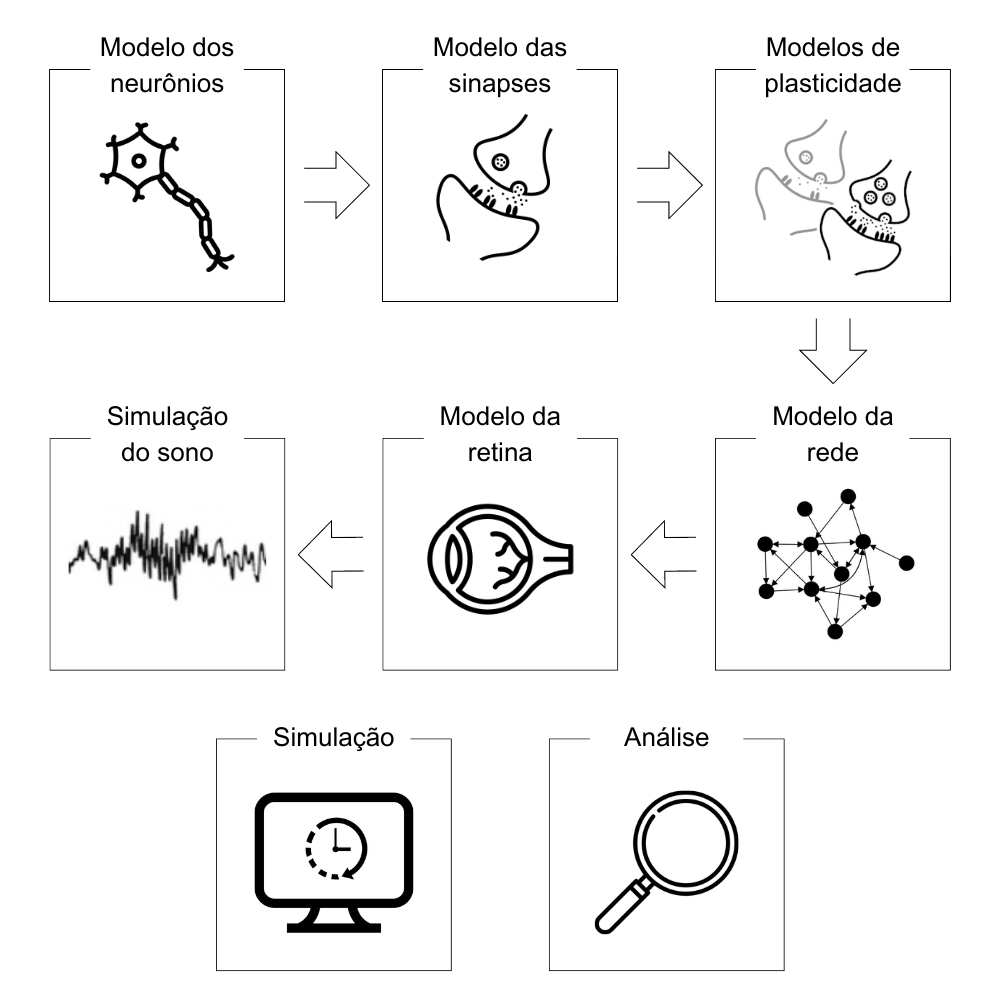
\includegraphics[width=\linewidth]{figuras/metodologia.png}\label{fig_metodologia}
% \fonte{}
}}
\end{figure}


\section{Modelo dos neurônios}

A unidade básica de uma RNP é o neurônio, então o primeiro passo para o modelo será a modelagem do neurônio. O modelo de neurônio
utilizado será o \textit{Leaky Integrate-and-Fire} (LIF) devido à sua simplicidade, que captura o comportamento geral de um
neurônio enquanto permite simulações rápidas de larga escala, como apresentado na Seção~\ref{section_modelos_neuronios}.

\section{Modelo das sinapses}

O próximo passo será simular como os neurônios interagem entre si. Para isso, será utilizado o modelo de sinapse de condução,
apresentado na Seção~\ref{subsection_modelos_sinapses}.

\section{Modelos de plasticidade}

As sinapses, porém, não serão estáticas e terão diversas formas de plasticidade simuladas. Todas as sinapses serão plásticas, de
acordo com os seguintes modelos de plasticidade: PCP, PDTD-E, heterossináptica e a induzida por transmissor, apresentados na
Seção~\ref{section_modelos_plasticidade}.

\section{Modelo de conexão da rede}

A rede será composta de 5.120 neurônios LIF, sendo 4.096 excitatórios e 1.024 inibitórios. Cada neurônio da rede será conectado a
de forma aleatória a 10\% dos neurônios da rede.

\section{Modelo da retina}

De modo a simular a entrada de estímulos visuais, será simulada uma retina. A retina será composta de 4.096 neurônios LIF, com
cada neurônio representando um pixel em uma imagem de 64$\times$64 pixels. Cada neurônio da RNP receberá conexões dos neurônios da
retina de uma área circular de raio 8, em que o centro do círculo é escolhido aleatoriamente para cada neurônio. As conexões da
retina com a RNP não serão plásticas.

Como explicado na Seção~\ref{section_experimento}, os estímulos serão imagens simples de serem reconhecidas, como formas
geométricas e símbolos. Essas imagens serão binárias: apenas preto e branco; o neurônio da retina correspondente a um pixel preto
irá disparar com frequência de 10Hz, enquanto o neurônio correspondente a um pixel branco irá disparar com frequência de 35Hz.

\section{Simulação do sono}

Para simular o sono, a rede funcionará de dois modos diferentes intercalados: um modo de atividade, em que a rede vai funcionar
normalmente enquanto recebe estímulos, e um modo de inatividade, em que será simulado o sono. 

Durante a fase de inatividade, nenhum estímulo será apresentado à rede, mas ela vai continuar sendo simulada normalmente. Além
disso, essa fase será dividida em subfases de acordo com as fases do sono real. Para simular cada fase do sono, os neurônios
receberão uma corrente sinusoidal de frequência e amplitude diferentes para cada fase de modo a tentar imitar os padrões de
atividade cerebral durante o sono observados em eletroencefalograma; também serão simulados outros sinais característicos do sono
de forma similar injetando corrente, como os fusos do sono que ocorrem durante a fase N2.

\section{Experimentos}\label{section_experimento}

Como forma de avaliar o modelo proposto serão conduzidos dois principais experimentos.

\subsection{Experimento 1: Formação de assembleias neuronais}

O primeiro experimento consiste em simular a RNP apresentando estímulos ao modelo de retina e analisar se a repetição dos
estímulos leva à formação de assembleias neuronais associadas a cada estímulo a longo prazo. Esses estímulos serão algumas imagens
simples de serem reconhecidas, como formas geométricas e símbolos. Os estímulos serão apresentados à rede de forma intercalada e
aleatória, também haverão momentos da simulação em que nenhum estímulo será apresentado. 

O objetivo desse experimento é ter uma base de comparação para o experimento 2. Espera-se que a repetição desses
estímulos durante o tempo de simulação da RNP leve à formação de assembleias neuronais associadas a cada estímulo.

\subsection{Experimento 2: Formação de assembleias neuronais com sono}

De forma similar ao experimento 1, o segundo experimento consiste em simular a RNP apresentando os mesmos estímulos, mas dessa vez
com a simulação de sono. O objetivo desse experimento é analisar se a simulação de sono tem algum efeito na formação de
assembleias neuronais. Espera-se que a simulação de sono leve à formação de assembleias neuronais mais rapidamente e que elas
durem mais tempo e sejam mais estáveis, bem como possa permitir o esquecimento de estímulos já não mais relevantes e a memorização
de mais estímulos.

\section{Análise}

A parte final do trabalho consistirá em analisar as diferentes simulações feitas e determinar se a simulação de sono teve algum
efeito na formação de assembleias neuronais. Para isso, antes de tudo é necessário um modo de identificar as assembleias neuronais
e quais neurônios pertencem a cada uma.

Para determinar quais neurônios pertencem à assembleia neuronal associada a um estímulo, será analisada a frequência de disparos de
cada neurônio no intervalo $3s < t < 3.5s$ após a apresentação do estímulo. Os neurônios que disparam com frequência maior que
10Hz serão considerados como pertencentes à assembleia neuronal associada a um estímulo.

Por fim, será analisado quanto tempo leva para a assembleia neuronal associada ser formada e quanto tempo ela dura nas diferentes
simulações.